

%\newcommand*{\ACM}{}%

\ifdefined\ACM

%\documentclass[sigplan,screen]{acmart}
\documentclass[manuscript,screen,review]{acmart}

\else
\documentclass{article}
\usepackage[utf8]{inputenc}
\usepackage[a4paper, total={6.5in, 10in} ]{geometry}
\usepackage{braket}
\usepackage{xcolor}
\usepackage{amsmath}
\usepackage{amssymb}
\usepackage{amsfonts}
\usepackage{graphicx}
\usepackage{svg}
\usepackage{float}
\usepackage{tikz}
\usetikzlibrary{patterns, shapes.arrows}
\usepackage{adjustbox}
\usepackage{tikz-network}
\usepackage[ruled,lined,linesnumbered]{algorithm2e}
\usepackage{multicol}
\usepackage[backend=biber,style=alphabetic,sorting=ynt]{biblatex}
\usepackage{xcolor}
\usepackage{pgfplots}
\DeclareUnicodeCharacter{2212}{−}
\usepgfplotslibrary{groupplots,dateplot}
\pgfplotsset{compat=newest}



\addbibresource{sample.bib} %Import the bibliography file

\fi
\begin{document}

\newcommand{\commentt}[1]{\textcolor{blue}{ \textbf{[COMMENT]} #1}}
\newcommand{\ctt}[1]{\commentt{#1}}
\newcommand{\prb}[1]{ \mathbf{Pr} \left[ {#1} \right]}
\newcommand{\onotation}[1]{\(\mathcal{O} \left( {#1}  \right) \)}
\newcommand{\ona}[1]{\onotation{#1}}
%\newcommand{\PSI}{{\ket{\psi}}}
%\newcommand{\LESn}{\ket{\psi_n}}
%\newcommand{\LESa}{\ket{\phi_n}}
%\newcommand{\LESs}{\frac{1}{\sqrt{n}}\sum_{i}{\ket{\left(0^{i}10^{n-i}\right)^{n}}}}
%\newcommand{\Hn}{\mathcal{H}_{n}}
%\newcommand{\Ep}{\frac{1}{\sqrt{2^n}}\sum^{2^n}_{x}{ \ket{xx}}}
%\newcommand{\HON}{\ket{\psi_{\text{honest}}}}
%\newcommand{\Lemma}{\paragraph{Lemma.}}
\newcommand{\Cpa}{[n, \rho n, \delta n]}
%\setlength{\columnsep}{0.6cm}
\newcommand{\Jvv}{ \bar{J_{v}} } 
\newcommand{\Cvv}{ \tilde{C_{v}} } 

\newcommand{\Gz}{ G_{z}^{\delta} } 
\newcommand{ \Tann } {  \mathcal{T}\left( G, C_0 \right) }


\title{Removing The $w$-Robustness Assumptions.} 
\author{David Ponarovsky}

\ifdefined\ACM
\affiliation{%
  \institution{The Th{\o}rv{\"a}ld Group}
  \streetaddress{1 Th{\o}rv{\"a}ld Circle}
  \city{Hekla}
  \country{Iceland}}
\email{larst@affiliation.org}
\else
\maketitle
\fi
\begin{abstract}
  Quantum feasibility hinges on the assumption that the basic gate's noise rate is below a certain threshold. Here we study the behavior of computation models when the noise is slightly greater than that threshold. In particular, We ask if one can design a fault tolerance schema such that if the noise is above the threshold, it is still grunted that the final generated state would have a value. 
\end{abstract}

\ifdefined\ACM
\maketitle
\fi
%\begin{multicols*}{2}
\section{Preambles}
  In this work, we propose a new construction for good LDPC codes, which also have a good testability parameter. In the sense that verfining a constant number of random checks, would be enough to detect any error with probability proportional to the error size. In contrast to previews, constructions made by \cite{Dinur}, \cite{leverrier2022quantum} and \cite{Pavel}, our construction doesn't require spicel properties of the small codes, such as $w$-robustness and $p$-resistance for puncturing. 
  
  Our proof also indirectly answers the following question. Why most of the good LDPC codes are known to be bad in terms of detecting errors? In other words, It seems that for most of them, there exist strings that are very far from being in the code and, meanwhile, fail to satisfy only a small number of restrictions.
  While the previous LDPC constructions focused on ensuring that the yielded code would have a good rate and distance parameters, our construction enforces the restrictions collection to have a nontrivial fraction of degeneration. That is, removing a single restriction will not change the code, as any restriction is linearly dependent on the others.



      \section{Introduction}
  %Coding theory has emerged by the need to transfer information in noisy communication channels. By embedding a message in higher dimension space, one can guarantee robustness against possible faults. The ratio of the original content length to the passed message \emph{length} is the \emph{rate} of the code, and it measures how consuming our communication protocol is. Furthermore, the \emph{distance} of the code quantifies how many faults the scheme can absorb such that the receiver can recover the original message. We could consider the code as all the strings that satisfy a specified restrictions collection.
%  
%
%  Non-formally, code is good if its distance and rate are scaled linearly in the encoded message length. In practice, one is also interested in implementing those checks efficiently. We say that a code is an LDPC if any bit is involved in a constant number of restrictions, each of which is a linear equation, and if any restriction contains a fixed number of variables.
%
%  Furthermore, finally, another characteristic of the code is its testability, which is the complexity of the number of random checks one should do to negate that a given candidate is in the code. Besides good codes being considered efficient in terms of robustness and overhead, they are also vital components in establishing secure multiparty computation \cite{MultiParty} and have a deep connection to probabilistic proofs.
%
%  First, we state the notations, definitions, and formal theorem in section 2. Then in sections 3 and 4, we review past results and provide their proofs to make this paper self-contained. Readers familiar with the basic concepts of LDPC, Tanner, and Expanders codes construction should consider skipping directly to section 5, in which we provide our proof. 
%

Coding theory has emerged due to the need to transfer information in noisy communication channels. By embedding a message in a higher-dimensional space, one can guarantee robustness against possible faults. The ratio of the original content length to the transmitted message \emph{length} is the \emph{rate} of the code, and it measures how consuming our communication protocol is. Additionally, the \emph{distance} of the code quantifies how many faults the scheme can absorb such that the receiver can recover the original message. We can consider the code as a collection of all strings that satisfy specified restrictions.

Non-formally, a code is good if its distance and rate scale linearly with the encoded message length. In practice, one is also interested in implementing these checks efficiently. We say that a code is an LDPC if any bit is involved in a constant number of restrictions, each of which is a linear equation, and if any restriction contains a fixed number of variables.

Moreover, another characteristic of the code is its testability, which is the complexity of the number of random checks one must do to verify that a given candidate is in the code. Besides being considered efficient in terms of robustness and overhead, good codes are also vital components in establishing secure multiparty computation \cite{MultiParty} and in the proof of the PCP theorem~\cite{PCPoriginal}.

%In Section 2, we state the notations, definitions, and formal theorem. Then, in Sections 3 and 4, we review past results and provide their proofs to make this paper self-contained. Readers familiar with the basic concepts of LDPC, Tanner, and Expanders codes construction may consider skipping directly to Section 5, in which we provide our proof.
%Readers familiar with the basic concepts of LDPC, Tanner, and Expanders codes construction may skip Sections 2, 3, and 4 and proceed directly to Section 5, where we provide our proof.

  %Linear Error Correction Codes, 
  \subsection{Notations, Definitions, And Our Contribution}
  Here we focus only on linear binary codes, which one could think about as linear subspaces of $\mathbb{F}_{2}^{n}$. A common way to measure resilience is to ask how many bits an evil entity needs to flip such that the corrupted vector will be closer to another vector in that space than the original one. Those ideas were formulated by Hamming \cite{Hamming}, who presented the following definitions. 
  \begin{definition} \label{bi-code} Let $n \in \mathbb{N}$ and $\rho, \delta\in \left( 0,1 \right)$. We say that $C$ is a \textbf{binary linear code} with parameters $[n, \rho n, \delta n]$. If $C$ is a subspace of $\mathbb{F}_{2}^{n}$, and the dimension of $C$ is at least $\rho n$. In addition, we call the vectors belong to $C$ \textit{codewords} and define the distance of $C$ to be the minimal number of different bits between any codewords pair of $C$.   
  \end{definition}
  From now on, we will use the term code to refer to linear binary codes, as we don't deal with any other types of codes. Also, even though it is customary to use the above parameters to analyze codes, we will use their percent forms called the relative distance and the rate of code, matching $\delta$ and $\rho$ correspondingly.     
  \begin{definition} \label{family} A \textbf{family of codes} is an infinite series of codes. Additionally, suppose the rates and relative distances converge into constant values $\rho,\delta$. In that case, we abuse the notation and call that family of codes a code with $[n, \rho n, \delta n]$ for fixed $\rho, \delta\in [ 0,1 )$, and infinite integers $n \in \mathbb{N}$.     
  \end{definition}
  Notice that the above definition contains codes with parameters attending to zero. From a practical view, it means that either we send too many bits, more than a constant amount, on each bit in the original message. Or that for big enough $n$, adversarial, limited to changing only a constant fraction of the bits, could disrupt the transmission. That distinction raises the definition of good codes.

  \begin{definition} \label{good-code} We will say that a family of codes is a \textbf{good code} if its parameters converge into positive values. 
  \end{definition}

  Apart from distance and rate here, we interest also that the checking process will be robust. In particular,  we wish that against significant errors, forgetting to perform a single check will sabotage the computation only with a tiny probability.  
  \begin{definition} \label{LTC} Consider a code $C$  a string $x$, and denote by $\xi\left( x \right)$ the fraction of the checks in which $x$ fails. $C$ will be called a \textbf{local-testability $f\left( n \right)$} If there exists $\kappa > 0$ such that 
  \begin{equation*}
    \begin{split}
      \frac{d\left( x, C \right)}{n} \le \kappa \cdot  \xi\left( x \right) f\left( n \right)
    \end{split}
  \end{equation*}
\end{definition}
  
  Nowadays, we are aware of a wide range of constructions yield good codes, including the expander codes of Sipser and Spilman \cite{ExpanderCodes} and the LTC codes of Dinur \cite{Dinur}, \cite{Pavel}, \cite{leverrier2022quantum}. Thus if a decade ago, the main question was the existence of a good code and its construction, now, and particularly in this work, we concentrate on getting a deep understanding of what makes those constructions work. By utilizing those insights, we succussed in achieving significantly simpler construction. Our results: 

 \begin{theorem*}[Theorem 1] There exist a constant $\alpha > 0$ and an infinte family of Tanner Codes $C = \Tann$ such that any ireducable codeword $x$ of a coresponding disagreement code $x \in C_{\oplus}$ at length $n$, weight at least $\alpha n$. \end{theorem*}

\begin{theorem*}[Theorem 1+] There exist a constant $\alpha > 0 $ and infinite familiy of codes which satesfies Theroem 1 and also good.
  \end{theorem*}




  \subsection{Singleton Bound}  
  To get a feeling of the behavior of the distance-rate trade-of, Let us consider the following two codes; each demonstrates a different extreme case. First, define the repetition code $C_{r} \subset \mathbb{F}_{2}^{n \cdot r}$, In which, for a fixed integer $r$, any bit of the original string is duplicated $r$ times. Second, consider the parity check code $C_{p} \subset \mathbb{F}_{2}^{n+1}$, in which its codewords are only the vectors with even parity. Let us analyze the repetition code. Clearly, any two $n$-bits different messages must have at least a single different bit. Therefore their corresponding encoded codewords have to differ in at least $r$ bits. Hence, by scaling $r$, one could achieve a higher distance as he wishes. Sadly the rate of the code decays as $n/nr = 1/r$. In contrast, the parity check code adds only a single extra bit for the original message. Therefore scaling $n$ gives a family which has a rate attends to $\rho \rightarrow 1$. However, flipping any two different bits of a valid codeword is conversing the parity and, as a result, leads to another valid codeword.

  To summarize the above, we have that, using a simple construction, one could construct the codes $[r, 1, r]$, $[r, r-1, 2]$. Each has a single perfect parameter, while the other decays to the worst. In the next section, we will review the Singleton bound, which states that for any code (not necessarily good), there must be a zero-sum game between the relative distance and the rate.
  Now, we are ready to formulate our contribution. 


  Besides being the first bound, Singleton bound demonstrates how one could get results by using relatively simple elementary arguments. It is also engaging to ask why the proof yields a bound that, empirically, seems far from being tight.
  \begin{theorem*}[Singleton Bound.]\label{theorem*:Sing}  For any linear code with parameter $[n,k,d]$, the following inequality holds:
  \begin{equation*}
    k+ d \le n + 1
  \end{equation*} 
  \end{theorem*}

\begin{proof} Since any two codewords of $C$ differ by at least $d$ coordinates, we know that by ignoring the first $d-1$ coordinate of any vector, we obtain a new code with one-to-one corresponding to the original code. In other words, we have found a new code with the same dimension embedded in $\mathbb{F}_{2}^{n-d+1}$. Combine the fact that dimension is, at most, the dimension of the container space, we get that:  
  \begin{equation*}
    \begin{split}
      \dim C &= 2^{k} \le 2^{n-d+1} \Rightarrow k+d \le n + 1
    \end{split}
  \end{equation*}
\end{proof}

It is also well known that the only binary codes that reach the bound are: $[n,1,n]$, $[n,n-1,2]$,$[n,n,1]$ \cite{eczoo_mds}. In particular, there are no good binary codes that obtain equality(And no binary code which get close to the equality exits). Let's review the polynomial code family \cite{Reed1960PolynomialCO}, which is a code over none binary field that achieve the Singleton Bound. 

\subsection{Polynomial Code}. Consider the field $\mathbb{F}_{m}$ for an arbitrary prime power $m=q^{l}$ greater than $n$. The polynomial codes relay on the fact that any two different polynomials in the ring $\mathbb{F}_{m}\left[ x \right]$ at degree at most $d$ different by at least $n - d + 1$ points. By define the code to be the subspace contains all the polynomials at degree at most $d$ encoded by $n$ numbers associated with their values. Formally we define:     
\begin{definition}
  Fix $m > n $ to be a prime power and let $a_{0},a_{1},a_{2},\ldots a_{n}$ distinct points of the field $\mathbb{F}_{m} = R$  and define the code $C \subset R $ as follows:  
  \begin{equation*}
    \begin{split}
      C = \left\{p\left(a_{0}\right),p\left(a_{1}\right),p\left(a_{2}\right),\cdots p\left(a_{n}\right) : p \text{ is polynomial at degree at most } k \right\}
    \end{split}
  \end{equation*}
\end{definition}
\ctt{ Add a statement about the vanishing rate of the binary encoded version. And add a paragraph about Tanner code in which each edge correspond to a non binary alpha-bet.  }
Next, we will review Tanner's construction, that in addition to being a critical element to our proof, also serves as an example of how one can construct a code with arbitrary length and positive rate.
  \subsection{Tanner Code}
  The constructions require two main ingredients: a graph $\Gamma$, and for simplicity, we will restrict ourselves to a $\Delta$ regular graph. Secondly, a small code $C_{0}$ at length equals the graph's regularity, namely $C_{0} = [\Delta,\rho\Delta, \delta\Delta]$. We can think about any bit string at length E as an assignment over the edges of the graph. Furthermore, for every vertex $v \in \Gamma$, we will call the bit string, which is set on its edges, the local view of $v$. Then we can define, \cite{Tanner}:
  \begin{definition}  Let $ C = \mathcal{T}\left( \Gamma, C_{0} \right)$  be all the codewords which, for any vertex $v\in \Gamma$, the local view of $v$ is a codeword of $C_{0}$. We say that $C$ is a \textbf{Tanner code}\label{Tan} of $\Gamma, C_{0}$. Notice that if $C_{0}$ is a binary linear code, So $C$ is.  
  \end{definition}

  It's also worth mentioning that the first construction of good classical codes, due to Sipser and Shpilman, are Tanner codes over expanders graphs \cite{ExpanderCodes}.
  \begin{theorem*}  Tanner codes have a rate of at least $2\rho - 1$. \end{theorem*}
  \begin{proof}  The dimension of the subspace is bounded by the dimension of the container minus the number of restrictions. So assuming non-degeneration of the small code restrictions, we have that any vertex count exactly $ \left( 1 - \rho  \right)\Delta $ restrictions. Hence, \begin{equation*}
    \begin{split}
      \dim C & \ge \frac{1}{2}n\Delta - \left( 1-\rho \right)\Delta n = \frac{1}{2}n\Delta\left( 2\rho - 1 \right)  
    \end{split}
  \end{equation*} Clearly, any small code with rate $> \frac{1}{2}$ will yield a code with an asymptotically positive rate \end{proof} 
  \subsubsection{Setting $C_{0}$ To Be The Polynomial Code.}
  
  \begin{equation*}
    \begin{split}
     \log \Delta \dim C & \ge \frac{1}{2}n\Delta  - \left( 1- \rho  \right) \Delta n = \frac{1}{2}n\Delta\left( 2\rho - 1 \right)  \\
     \Rightarrow  \dim C & \ge \frac{1}{\log \Delta} \frac{1}{2}n\Delta\left( 2\rho - 1 \right)  
    \end{split}
  \end{equation*}
  \subsection{Expander Codes}
  We saw how a graph could give us arbitrarily long codes with a positive rate. We will show, Sipser's result that if the graph is also an expander, we can guarantee a positive relative distance. We notice that the name expander codes is coined for a more general version than the one we will present.   
  \begin{definition} Denote by $\lambda$ the second eigenvalue of the adjacency matrix of the $\Delta$-regular graph. For our uses, it will be satisfied to define expander as a graph $G = \left( V,E \right)$ such that for any two subsets of vertices $T,S \subset V$, the number of edges between $S$ and $T$ is at most:
  \begin{equation*}
    \begin{split}
      \mid E\left( S,T \right) - \frac{\Delta}{n}|S||T| \mid \le \lambda\sqrt{|S| |T|} 
    \end{split}
  \end{equation*}
\end{definition}
This bound is known as the Expander Mixining Lemma. We refer the reader to \cite{hoory2006expander} for more deatilied survery. 
  \begin{theorem*} Theorem, let $C$ be the Tanner Code defined by the small code $C_{0} = [\Delta,\delta\Delta, \rho\Delta ]$ such that $\rho \ge \frac{1}{2}$ and the expander graph $G$ such that $\delta\Delta \ge \lambda$. $C$ is a good  LDPC code.
  \end{theorem*}
  \begin{proof} We have already shown that the graph has a positive rate due to the Tunner construction. So it's left to show also the code has a linear distance. Fix a codeword $x \in C$ and denote By $S$ the support of $x$ over the edges. Namely, a vertex $v\in V$ belongs to $S$ if it connects to nonzero edges regarding the assignment by $x$, Assume towards contradiction that $|x| = o\left( n \right)$. And notice that $|S|$ is at most $2|x|$, Then by The Expander Mixining Lemma we have that: 
  \begin{equation*}
    \begin{split}
      \frac{E\left( S,S \right)}{|S|} & \le \frac{\Delta}{n}|S|  + \lambda \\
      & \le_{ n \rightarrow \infty} o\left( 1 \right) + \lambda
    \end{split}
  \end{equation*}

  Namely, for any such sublinear weight string, $x$, the average of nontrivial edges for the vertex is less than $\lambda$. So there must be at least one vertex $v \in S$ that, on his local view, sets a  string at a weight less than $\lambda$. By the definition of $S$, this string cannot be trivial. Combining the fact that any nontrivial codeword of the $C_{0}$ is at weight at least $\delta\Delta$, we get a contradiction to the assumption that $v$ is satisfied, videlicet, $x$ can't be a codeword \end{proof}
 


 \subsection{Tanner testability.} This subsection will explain why testability is so hard to achieve. Let $C$ be a good Tanner expander code as defined above. And consider an arbitrary vertex $u \in V$ and arbitrary restriction of $C_{0}$, $h$. Now define $\tilde{C}$ as the code obtained by requiring all the restrictions of $C$ except $h$ on $u$. That it, $u$ is satisfied if his local view satisfies all the $C_{0}$ restrictions apart from $h$.
  Also, for convenience, denote the small code $u$ enforces on his local view by $C_{0}^{u}$. Let us assume that the distance of $C_{0}^{u}$ is at least $\delta\Delta$. 
  Then, by repeating almost exactly the steps above with caution, one could prove that $\tilde{C}$ also has a linear distance. 


  Assume that $\tilde{C} \neq C \Rightarrow$ there exists $x\in \tilde{C} / C$. By definition, for any $v\in V / \{u\}$ it holdes that $x|_{v} \in C_{0}$. Hence, the assumption that $ x \notin C$  implies $x|_{u} \notin C_{0}$ So, clearly, $x$ fails at a constant number of $C$'s checks. On the other hand, the closest codeword $y \in C$ to $x$ is also a codeword of $\tilde{C}$ as $y|_{v} \in C_{0}$ for every $v\in V$.  Hence:
  \begin{equation*}
    \begin{split}
      d\left( x,C \right) &= d\left( x,y \right) \ge d\left( \tilde{C} \right) =\Theta\left( n \right)
    \end{split}
  \end{equation*}
  Even if a linear number of bits needed to be flipped to correct $x$, only a single check observes that $x$ is indeed an error.
  \section{Construction}
  \subsection{ Almost LTC With Zero Rate}
  \paragraph{Definition. The Disagreement Code.} Given a Tanner code $C = \Tann$, define the code $C_{\oplus}$ to contain all the words equal to the formal summation $ \sum_{v \in V\left( G \right)} {c_{v} }$ when $c_{v}$ is an assignment of a codeword $ c_{v} \in C_0 $  on the edges of the vertex $ v \in V\left( G \right)$.
  We call to such code the \textit{disagreement code} of $C$, as edges are set to 1 only if their connected vertices contribute to the summation codewords that are different on the corresponding bit to that edge. In addition, we will call to any contribute $c_v$, the \textit{suggestion} of $v$. And notice that by linearity, each vertex suggests, at most, a single suggestion.   


  Finally, given a bits assessment $x \in \mathbb{F}_{2}^{E}$ over the edges of $G$, we will denote by $x^{\oplus} \in C_{\oplus} $ the codeword which obtained by summing up suggestions set such each vertex suggests the closet codeword to his local view. Namely, for each $v \in V$ define:   
  \begin{equation*}
    \begin{split}
      c_{v} & \leftarrow \arg_{ \tilde{c} \in C_{0}} \min{ d( x|_{v} , \tilde{c} ) } \ \ \forall v\in V   \\
      x^{\oplus} & \leftarrow \sum_{v \in V}{c_{v}} 
    \end{split}
  \end{equation*}
  We will think about $x^{\oplus}$ as the disagreement between the vertices over $x$. 


  \paragraph{Lemma. Linearity Of The Disagreement.} Consider the code $C = \Tann$. Let $ x \in \mathbb{F}_{2}^{E}$ then for any $ y \in C$ it holds that: 
  \begin{equation*}
    \begin{split}
      \left( x + y  \right)^{\oplus} = \left( x  \right)^{\oplus} 
    \end{split}
  \end{equation*}
  \paragraph{Proof.} Having that $y \in C$ followes $y|_v \in C_{0}$ and therefore $\arg_{ \tilde{c} \in C_{0}} \min{ d( z  , \tilde{c} ) } = y|_{v} + \arg_{ \tilde{c} \in C_{0}} \min{ d( z, \tilde{c} + y|_{v} ) } $, Hence the suggestion made by vertrx $v$ is: 
  \begin{equation*}
    \begin{split}
      c_{v}\leftarrow &  \arg_{ \tilde{c} \in C_{0}} \min{ d( (x+y)|_{v}  , \tilde{c} ) } \\
      \leftarrow &  y|_{v} +  \arg_{ \tilde{c} \in C_{0}} \min{ d( (x+y)|_{v}  , \tilde{c} + y|_{v} ) } \\
      \leftarrow &  y|_{v} +  \arg_{ \tilde{c} \in C_{0}} \min{ d( x|_{v} , \tilde{c} ) } 
    \end{split}
  \end{equation*}
  It follows that: 

  \begin{equation*}
    \begin{split}
      \left( x + y \right)^{\oplus} =& \sum_{v\in V}{c_{v}} = \sum_{v \in V}{y|_{v}} + \sum_{v\in V}{ \arg_{ \tilde{c} \in C_{0}} \min{ d( x|_{v} , \tilde{c} ) } } \\ 
      =& y^{\oplus} + x^{\oplus} = x^{\oplus}
    \end{split}
  \end{equation*}
  When the last transition follows immediately by the fact that $y \in C$ and therefore any pair of connected vertices contribute the same value for their associated edge \end{proof}

  \paragraph{Definition.} Let $C = \Tann$. We say that $x \in C_{\oplus}$ is \textit{reducable} if there exists a vertex $v$ and a small codeword $c_v$, for which, adding the assignment of $c_v$ over the $v$'s edges to $x$ decreases the weight. Namely, $|x + c_{v}| < |x|$. If $x \in C_{\oplus}$ is not a reducable codeword then we say that $x$ is \textit{ireducable}.   

  \paragraph{Theorem 1.} There exist a constant $\alpha > 0$ and an infinte family of Tanner Codes $C = \Tann$ such that any ireducable codeword $x$ of a coresponding disagreement code $x \in C_{\oplus}$ at length $n$, weight at least $\alpha n$.
  \paragraph{Proof.} By induction over the number of vertices $V^\prime \subset V$, which suggest a nontrivial codeword to $x$. Base, assume that a single vertex $v \in V$ suggests a nontrivial codeword $c_{v} \in C_{0}$. Then it's clear that $x = c_{v}$. And therefore, we have that $|x +c_{v}| = 0 < |x|$.

  Assume the correctness of the argument for every codeword defined by at most $m$ nontrivial suggestions made by $V^\prime \subset V$. And consider the graph $\left( V^\prime, E^\prime \right)$ induced by them. If the graph has more than a single connectivity component, then any of them is also a codeword of $C_{\oplus}$  but composed of at most $m-1$ nontrivial suggestions. Therefore, by the assumption, we could find a vertex $v$ and a proper small codeword $c_v \in C_0 $, such that the addition of the suggestion will decrease the weight of the codeword defined on that component and therefore decrease the total weight of $x$.

  So, we can assume that the vertices in $V^\prime$ compose a single connectivity component. Let be $x|_{v} \in \mathbb{F}_{2}^{\Delta}$ the bits of $x$ on the indices corresponding to $v$'s edges. If there is any $v$, with suggestion $c_{v}$, such that $ \frac{1}{2}w\left( c_{v}\right) < w\left( x|_{v} \right)$, then we could pick to turn on $c_{v}$ again and have that:
  \begin{equation*}
    \begin{split}
      |x+c_{v}| & = | x_{/v} + x_{v} + c_{v}| = |x_{/v}| + w\left( c_{v} \right) + w\left( x|_{v} \right) \\
      & < |x_{/v}| + \frac{1}{2}w\left( c_{v} \right) \le |x_{/v}| + w\left( x|_{v} \right) = |x|
    \end{split}
  \end{equation*}

  Hence it is left to consider the case that for any $v\in V^\prime$, it holds that $\frac{1}{2}w\left( c_{v}\right) >  w\left( x|_{v} \right)$ (Notice that if they equal, then by turn on $c_{v}$, we back again to codeword made by $m-1$ nontrivial suggestions). We will prove that this case is possible only for codewords with wight at least $\alpha|E|^{1-\varepsilon}$.

  For any $S \subset E$, define $w_{S}\left( x \right)$ as the weight that $x$ induces over $S$. And notice that any edge of $E$ connected only to a single vertex in $V^\prime$ equals the corresponding bit in the original suggestion made by $c_{v}$. Hence for every $v\in V^\prime$, it holds that $w_{E / E^\prime}\left(x|_{v}\right) = w_{E / E^\prime}\left(c_{v}\right)$. 

%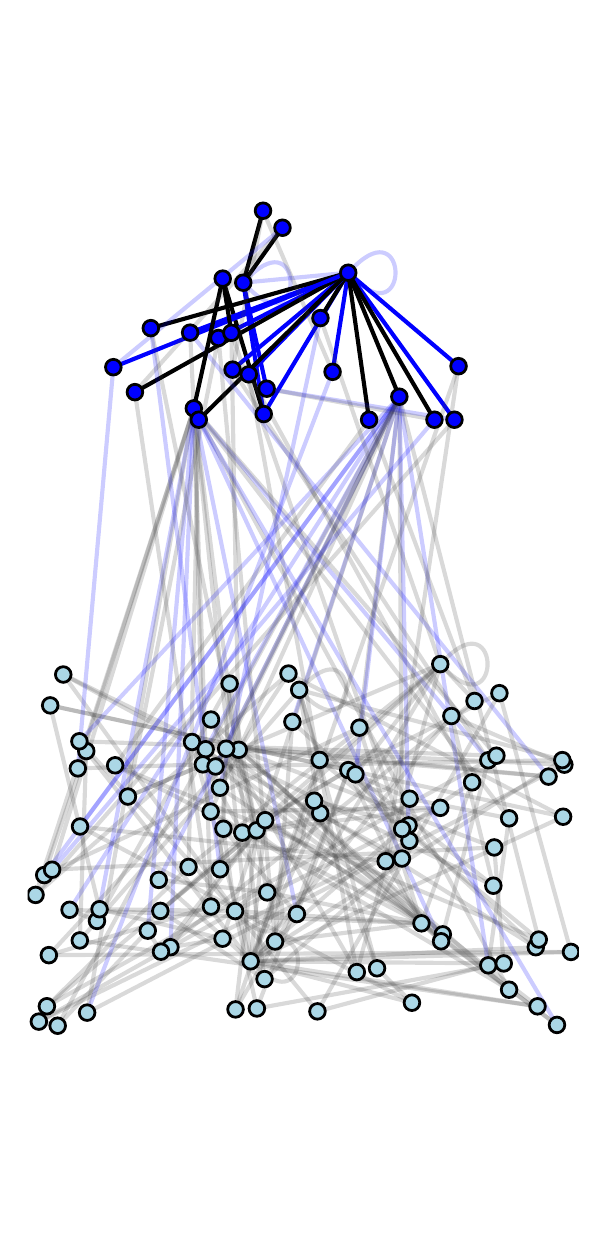
\begin{tikzpicture}
\clip (0,0) rectangle (7.0,15.0);
\Vertex[x=2.738,y=11.761,size=0.1,color=blue]{0}
\Vertex[x=2.998,y=10.093,size=0.1,color=blue]{119}
\Vertex[x=4.071,y=11.888,size=0.1,color=blue]{1}
\Vertex[x=2.063,y=11.127,size=0.1,color=blue]{2}
\Vertex[x=6.615,y=5.488,size=0.1]{3}
\Vertex[x=2.110,y=10.165,size=0.1,color=blue]{64}
\Vertex[x=2.087,y=5.928,size=0.1]{4}
\Vertex[x=2.681,y=5.829,size=0.1]{9}
\Vertex[x=2.725,y=4.777,size=0.1]{5}
\Vertex[x=2.832,y=3.143,size=0.1]{16}
\Vertex[x=5.240,y=5.092,size=0.1]{6}
\Vertex[x=4.072,y=5.571,size=0.1]{25}
\Vertex[x=2.324,y=5.044,size=0.1]{7}
\Vertex[x=2.634,y=3.781,size=0.1]{96}
\Vertex[x=6.114,y=2.782,size=0.1]{8}
\Vertex[x=4.720,y=10.313,size=0.1,color=blue]{49}
\Vertex[x=1.273,y=5.235,size=0.1]{10}
\Vertex[x=2.907,y=4.806,size=0.1]{81}
\Vertex[x=2.423,y=11.059,size=0.1,color=blue]{11}
\Vertex[x=5.240,y=6.917,size=0.1]{40}
\Vertex[x=3.142,y=3.394,size=0.1]{12}
\Vertex[x=3.362,y=6.184,size=0.1]{13}
\Vertex[x=5.001,y=3.625,size=0.1]{24}
\Vertex[x=6.453,y=3.322,size=0.1]{14}
\Vertex[x=3.715,y=5.024,size=0.1]{15}
\Vertex[x=3.448,y=6.590,size=0.1]{105}
\Vertex[x=1.665,y=4.177,size=0.1]{17}
\Vertex[x=3.042,y=4.018,size=0.1]{18}
\Vertex[x=1.564,y=11.184,size=0.1,color=blue]{19}
\Vertex[x=2.443,y=4.312,size=0.1]{20}
\Vertex[x=2.565,y=6.669,size=0.1]{21}
\Vertex[x=0.880,y=3.656,size=0.1]{22}
\Vertex[x=0.532,y=3.797,size=0.1]{23}
\Vertex[x=3.016,y=4.935,size=0.1]{26}
\Vertex[x=5.272,y=3.485,size=0.1]{27}
\Vertex[x=5.850,y=5.696,size=0.1]{28}
\Vertex[x=2.602,y=10.657,size=0.1,color=blue]{29}
\Vertex[x=2.989,y=12.675,size=0.1,color=blue]{30}
\Vertex[x=3.872,y=10.629,size=0.1,color=blue]{31}
\Vertex[x=0.755,y=2.491,size=0.1]{32}
\Vertex[x=6.816,y=5.640,size=0.1]{33}
\Vertex[x=5.381,y=6.258,size=0.1]{34}
\Vertex[x=5.914,y=4.103,size=0.1]{35}
\Vertex[x=0.452,y=6.785,size=0.1]{36}
\Vertex[x=4.753,y=4.448,size=0.1]{37}
\Vertex[x=3.008,y=2.917,size=0.1]{38}
\Vertex[x=1.685,y=3.783,size=0.1]{39}
\Vertex[x=3.718,y=11.312,size=0.1,color=blue]{41}
\Vertex[x=2.442,y=5.347,size=0.1]{42}
\Vertex[x=2.260,y=5.836,size=0.1]{43}
\Vertex[x=6.475,y=2.571,size=0.1]{44}
\Vertex[x=0.662,y=3.408,size=0.1]{45}
\Vertex[x=0.744,y=5.813,size=0.1]{46}
\Vertex[x=0.210,y=4.238,size=0.1]{47}
\Vertex[x=4.213,y=6.110,size=0.1]{48}
\Vertex[x=4.163,y=5.517,size=0.1]{50}
\Vertex[x=4.851,y=5.208,size=0.1]{51}
\Vertex[x=6.114,y=4.959,size=0.1]{52}
\Vertex[x=5.850,y=3.092,size=0.1]{53}
\Vertex[x=3.680,y=2.507,size=0.1]{54}
\Vertex[x=5.991,y=6.548,size=0.1]{55}
\Vertex[x=6.900,y=3.262,size=0.1]{56}
\Vertex[x=0.269,y=3.221,size=0.1]{57}
\Vertex[x=2.328,y=3.838,size=0.1]{58}
\Vertex[x=1.362,y=10.371,size=0.1,color=blue]{59}
\Vertex[x=3.236,y=12.459,size=0.1,color=blue]{60}
\Vertex[x=1.088,y=10.688,size=0.1,color=blue]{61}
\Vertex[x=0.637,y=5.593,size=0.1]{62}
\Vertex[x=2.225,y=5.644,size=0.1]{63}
\Vertex[x=3.419,y=3.743,size=0.1]{65}
\Vertex[x=2.486,y=4.826,size=0.1]{66}
\Vertex[x=2.521,y=5.843,size=0.1]{67}
\Vertex[x=5.250,y=3.397,size=0.1]{68}
\Vertex[x=2.328,y=6.213,size=0.1]{69}
\Vertex[x=4.180,y=3.006,size=0.1]{70}
\Vertex[x=2.808,y=10.597,size=0.1,color=blue]{71}
\Vertex[x=5.644,y=5.416,size=0.1]{72}
\Vertex[x=4.837,y=4.869,size=0.1]{73}
\Vertex[x=3.638,y=5.182,size=0.1]{74}
\Vertex[x=4.437,y=3.054,size=0.1]{75}
\Vertex[x=4.880,y=2.617,size=0.1]{76}
\Vertex[x=0.665,y=4.855,size=0.1]{77}
\Vertex[x=4.547,y=4.414,size=0.1]{78}
\Vertex[x=5.472,y=10.701,size=0.1,color=blue]{79}
\Vertex[x=2.640,y=2.532,size=0.1]{80}
\Vertex[x=1.813,y=3.322,size=0.1]{82}
\Vertex[x=2.475,y=3.430,size=0.1]{83}
\Vertex[x=0.913,y=3.804,size=0.1]{84}
\Vertex[x=0.286,y=6.393,size=0.1]{85}
\Vertex[x=6.800,y=4.979,size=0.1]{86}
\Vertex[x=3.312,y=6.797,size=0.1]{87}
\Vertex[x=0.100,y=3.986,size=0.1]{88}
\Vertex[x=5.420,y=10.021,size=0.1,color=blue]{89}
\Vertex[x=3.035,y=10.415,size=0.1,color=blue]{90}
\Vertex[x=5.166,y=10.021,size=0.1,color=blue]{91}
\Vertex[x=0.310,y=4.306,size=0.1]{92}
\Vertex[x=5.925,y=4.589,size=0.1]{93}
\Vertex[x=6.046,y=3.116,size=0.1]{94}
\Vertex[x=2.911,y=2.544,size=0.1]{95}
\Vertex[x=0.657,y=5.937,size=0.1]{97}
\Vertex[x=5.953,y=5.754,size=0.1]{98}
\Vertex[x=0.244,y=2.572,size=0.1]{99}
\Vertex[x=2.043,y=4.341,size=0.1]{100}
\Vertex[x=2.173,y=10.021,size=0.1,color=blue]{101}
\Vertex[x=6.722,y=2.335,size=0.1]{102}
\Vertex[x=2.386,y=5.617,size=0.1]{103}
\Vertex[x=6.790,y=5.698,size=0.1]{104}
\Vertex[x=3.708,y=5.700,size=0.1]{106}
\Vertex[x=6.491,y=3.419,size=0.1]{107}
\Vertex[x=1.111,y=5.632,size=0.1]{108}
\Vertex[x=4.336,y=10.021,size=0.1,color=blue]{109}
\Vertex[x=5.675,y=6.449,size=0.1]{110}
\Vertex[x=1.693,y=3.265,size=0.1]{111}
\Vertex[x=1.525,y=3.532,size=0.1]{112}
\Vertex[x=0.381,y=2.325,size=0.1]{113}
\Vertex[x=0.142,y=2.377,size=0.1]{114}
\Vertex[x=4.848,y=4.673,size=0.1]{115}
\Vertex[x=4.756,y=4.823,size=0.1]{116}
\Vertex[x=2.587,y=11.125,size=0.1,color=blue]{117}
\Vertex[x=2.477,y=11.813,size=0.1,color=blue]{118}
\Edge[,color=blue,opacity=1](0)(119)
\Edge[,color=blue,opacity=0.2](0)(1)
\Edge[,color=blue,opacity=0.2](0)(0)
\Edge[,color=black,opacity=1](0)(30)
\Edge[,color=black,opacity=1](0)(60)
\Edge[,color=blue,opacity=1](0)(90)
\Edge[,color=black,opacity=1](119)(118)
\Edge[,color=blue,opacity=1](119)(1)
\Edge[,color=blue,opacity=1](1)(2)
\Edge[,color=blue,opacity=0.2](1)(1)
\Edge[,color=blue,opacity=1](1)(11)
\Edge[,color=black,opacity=1](1)(19)
\Edge[,color=blue,opacity=1](1)(29)
\Edge[,color=blue,opacity=1](1)(31)
\Edge[,color=black,opacity=1](1)(41)
\Edge[,color=black,opacity=1](1)(49)
\Edge[,color=black,opacity=1](1)(59)
\Edge[,color=blue,opacity=1](1)(61)
\Edge[,color=blue,opacity=1](1)(71)
\Edge[,color=blue,opacity=1](1)(79)
\Edge[,color=blue,opacity=1](1)(89)
\Edge[,color=black,opacity=1](1)(91)
\Edge[,color=black,opacity=1](1)(101)
\Edge[,color=black,opacity=1](1)(109)
\Edge[,color=blue,opacity=0.2](2)(3)
\Edge[,opacity=0.2](2)(64)
\Edge[,opacity=0.2](3)(4)
\Edge[,opacity=0.2](3)(9)
\Edge[,opacity=0.2](64)(8)
\Edge[,color=blue,opacity=0.2](64)(22)
\Edge[,color=blue,opacity=0.2](64)(28)
\Edge[,opacity=0.2](64)(32)
\Edge[,opacity=0.2](64)(38)
\Edge[,opacity=0.2](64)(52)
\Edge[,opacity=0.2](64)(58)
\Edge[,opacity=0.2](64)(62)
\Edge[,opacity=0.2](64)(63)
\Edge[,color=blue,opacity=0.2](64)(65)
\Edge[,opacity=0.2](64)(16)
\Edge[,color=blue,opacity=0.2](64)(68)
\Edge[,color=blue,opacity=0.2](64)(82)
\Edge[,opacity=0.2](64)(88)
\Edge[,opacity=0.2](64)(92)
\Edge[,opacity=0.2](64)(98)
\Edge[,color=blue,opacity=0.2](64)(112)
\Edge[,color=black,opacity=1](64)(118)
\Edge[,opacity=0.2](4)(5)
\Edge[,opacity=0.2](4)(16)
\Edge[,opacity=0.2](9)(8)
\Edge[,opacity=0.2](9)(10)
\Edge[,opacity=0.2](9)(81)
\Edge[,opacity=0.2](9)(27)
\Edge[,opacity=0.2](9)(33)
\Edge[,opacity=0.2](9)(57)
\Edge[,opacity=0.2](9)(63)
\Edge[,opacity=0.2](9)(87)
\Edge[,opacity=0.2](9)(93)
\Edge[,opacity=0.2](9)(117)
\Edge[,opacity=0.2](5)(6)
\Edge[,opacity=0.2](5)(25)
\Edge[,opacity=0.2](16)(14)
\Edge[,opacity=0.2](16)(15)
\Edge[,opacity=0.2](16)(17)
\Edge[,opacity=0.2](16)(16)
\Edge[,opacity=0.2](16)(26)
\Edge[,opacity=0.2](16)(34)
\Edge[,opacity=0.2](16)(44)
\Edge[,opacity=0.2](16)(46)
\Edge[,opacity=0.2](16)(56)
\Edge[,opacity=0.2](16)(74)
\Edge[,opacity=0.2](16)(76)
\Edge[,opacity=0.2](16)(86)
\Edge[,opacity=0.2](16)(94)
\Edge[,opacity=0.2](16)(104)
\Edge[,opacity=0.2](16)(106)
\Edge[,opacity=0.2](16)(116)
\Edge[,opacity=0.2](6)(7)
\Edge[,opacity=0.2](6)(96)
\Edge[,opacity=0.2](25)(24)
\Edge[,opacity=0.2](25)(26)
\Edge[,opacity=0.2](25)(25)
\Edge[,opacity=0.2](25)(35)
\Edge[,opacity=0.2](25)(55)
\Edge[,opacity=0.2](25)(65)
\Edge[,opacity=0.2](25)(85)
\Edge[,opacity=0.2](25)(95)
\Edge[,opacity=0.2](25)(115)
\Edge[,opacity=0.2](7)(8)
\Edge[,opacity=0.2](7)(49)
\Edge[,opacity=0.2](96)(24)
\Edge[,opacity=0.2](96)(36)
\Edge[,opacity=0.2](96)(54)
\Edge[,opacity=0.2](96)(66)
\Edge[,opacity=0.2](96)(84)
\Edge[,opacity=0.2](96)(95)
\Edge[,opacity=0.2](96)(97)
\Edge[,opacity=0.2](96)(96)
\Edge[,opacity=0.2](96)(114)
\Edge[,color=blue,opacity=0.2](49)(13)
\Edge[,color=blue,opacity=0.2](49)(17)
\Edge[,color=blue,opacity=0.2](49)(23)
\Edge[,opacity=0.2](49)(37)
\Edge[,color=blue,opacity=0.2](49)(43)
\Edge[,color=blue,opacity=0.2](49)(47)
\Edge[,opacity=0.2](49)(48)
\Edge[,color=blue,opacity=0.2](49)(50)
\Edge[,color=blue,opacity=0.2](49)(53)
\Edge[,opacity=0.2](49)(67)
\Edge[,color=blue,opacity=0.2](49)(73)
\Edge[,color=blue,opacity=0.2](49)(77)
\Edge[,opacity=0.2](49)(83)
\Edge[,color=blue,opacity=0.2](49)(97)
\Edge[,opacity=0.2](49)(103)
\Edge[,opacity=0.2](49)(107)
\Edge[,opacity=0.2](49)(113)
\Edge[,opacity=0.2](10)(11)
\Edge[,opacity=0.2](10)(40)
\Edge[,opacity=0.2](81)(21)
\Edge[,opacity=0.2](81)(39)
\Edge[,opacity=0.2](81)(51)
\Edge[,opacity=0.2](81)(69)
\Edge[,opacity=0.2](81)(80)
\Edge[,opacity=0.2](81)(82)
\Edge[,opacity=0.2](81)(81)
\Edge[,opacity=0.2](81)(99)
\Edge[,opacity=0.2](81)(111)
\Edge[,opacity=0.2](11)(12)
\Edge[,opacity=0.2](40)(20)
\Edge[,opacity=0.2](40)(39)
\Edge[,opacity=0.2](40)(41)
\Edge[,opacity=0.2](40)(40)
\Edge[,opacity=0.2](40)(50)
\Edge[,opacity=0.2](40)(70)
\Edge[,opacity=0.2](40)(80)
\Edge[,opacity=0.2](40)(100)
\Edge[,opacity=0.2](40)(110)
\Edge[,opacity=0.2](12)(13)
\Edge[,opacity=0.2](12)(24)
\Edge[,opacity=0.2](13)(14)
\Edge[,opacity=0.2](24)(18)
\Edge[,opacity=0.2](24)(23)
\Edge[,opacity=0.2](24)(42)
\Edge[,opacity=0.2](24)(48)
\Edge[,opacity=0.2](24)(72)
\Edge[,opacity=0.2](24)(78)
\Edge[,opacity=0.2](24)(102)
\Edge[,opacity=0.2](24)(108)
\Edge[,opacity=0.2](14)(15)
\Edge[,opacity=0.2](15)(105)
\Edge[,opacity=0.2](105)(45)
\Edge[,opacity=0.2](105)(75)
\Edge[,opacity=0.2](105)(104)
\Edge[,opacity=0.2](105)(106)
\Edge[,opacity=0.2](105)(105)
\Edge[,opacity=0.2](17)(18)
\Edge[,opacity=0.2](18)(19)
\Edge[,color=blue,opacity=0.2](19)(20)
\Edge[,opacity=0.2](20)(21)
\Edge[,opacity=0.2](21)(22)
\Edge[,opacity=0.2](22)(23)
\Edge[,opacity=0.2](26)(27)
\Edge[,opacity=0.2](27)(28)
\Edge[,opacity=0.2](28)(29)
\Edge[,opacity=0.2](29)(30)
\Edge[,opacity=0.2](30)(31)
\Edge[,color=blue,opacity=0.2](31)(32)
\Edge[,opacity=0.2](32)(33)
\Edge[,opacity=0.2](33)(34)
\Edge[,opacity=0.2](34)(35)
\Edge[,opacity=0.2](35)(36)
\Edge[,opacity=0.2](36)(37)
\Edge[,opacity=0.2](37)(38)
\Edge[,opacity=0.2](38)(39)
\Edge[,color=blue,opacity=0.2](41)(42)
\Edge[,opacity=0.2](42)(43)
\Edge[,opacity=0.2](43)(44)
\Edge[,opacity=0.2](44)(45)
\Edge[,opacity=0.2](45)(46)
\Edge[,opacity=0.2](46)(47)
\Edge[,opacity=0.2](47)(48)
\Edge[,opacity=0.2](50)(51)
\Edge[,opacity=0.2](51)(52)
\Edge[,opacity=0.2](52)(53)
\Edge[,opacity=0.2](53)(54)
\Edge[,opacity=0.2](54)(55)
\Edge[,opacity=0.2](55)(56)
\Edge[,opacity=0.2](56)(57)
\Edge[,opacity=0.2](57)(58)
\Edge[,opacity=0.2](58)(59)
\Edge[,opacity=0.2](59)(60)
\Edge[,color=blue,opacity=0.2](60)(61)
\Edge[,color=blue,opacity=0.2](61)(62)
\Edge[,opacity=0.2](62)(63)
\Edge[,opacity=0.2](65)(66)
\Edge[,opacity=0.2](66)(67)
\Edge[,opacity=0.2](67)(68)
\Edge[,opacity=0.2](68)(69)
\Edge[,opacity=0.2](69)(70)
\Edge[,opacity=0.2](70)(71)
\Edge[,opacity=0.2](71)(72)
\Edge[,opacity=0.2](72)(73)
\Edge[,opacity=0.2](73)(74)
\Edge[,opacity=0.2](74)(75)
\Edge[,opacity=0.2](75)(76)
\Edge[,opacity=0.2](76)(77)
\Edge[,opacity=0.2](77)(78)
\Edge[,opacity=0.2](78)(79)
\Edge[,opacity=0.2](79)(80)
\Edge[,opacity=0.2](82)(83)
\Edge[,opacity=0.2](83)(84)
\Edge[,opacity=0.2](84)(85)
\Edge[,opacity=0.2](85)(86)
\Edge[,opacity=0.2](86)(87)
\Edge[,opacity=0.2](87)(88)
\Edge[,opacity=0.2](88)(89)
\Edge[,color=blue,opacity=0.2](89)(90)
\Edge[,opacity=0.2](90)(91)
\Edge[,color=blue,opacity=0.2](91)(92)
\Edge[,opacity=0.2](92)(93)
\Edge[,opacity=0.2](93)(94)
\Edge[,opacity=0.2](94)(95)
\Edge[,opacity=0.2](97)(98)
\Edge[,opacity=0.2](98)(99)
\Edge[,opacity=0.2](99)(100)
\Edge[,opacity=0.2](100)(101)
\Edge[,color=blue,opacity=0.2](101)(102)
\Edge[,opacity=0.2](102)(103)
\Edge[,opacity=0.2](103)(104)
\Edge[,opacity=0.2](106)(107)
\Edge[,opacity=0.2](107)(108)
\Edge[,opacity=0.2](108)(109)
\Edge[,opacity=0.2](109)(110)
\Edge[,opacity=0.2](110)(111)
\Edge[,opacity=0.2](111)(112)
\Edge[,opacity=0.2](112)(113)
\Edge[,opacity=0.2](113)(114)
\Edge[,opacity=0.2](114)(115)
\Edge[,opacity=0.2](115)(116)
\Edge[,opacity=0.2](116)(117)
\Edge[,color=black,opacity=1](117)(118)
\end{tikzpicture}

  \begin{claim} For any $v \in V^\prime$ and corresponded suggestion $c_{v}$ it holds that: $w_{E^\prime}\left( c_{v} \right) \ge \frac{1}{2}\delta_{0}\Delta$. \end{claim}
  \begin{proof}By using the previews insight we get: \begin{equation*}
    \begin{split}
      w_{E^\prime}\left( c_{v} \right) &= w\left( c_{v} \right) - w_{E / E^\prime}\left( c_{v} \right) =  w\left( c_{v} \right) - w_{E / E^\prime}\left( x|_{v} \right) \\ 
      & \ge  w\left( c_{v} \right) - w\left( x|_{v} \right) \ge \frac{1}{2}w\left( c_{v} \right) = \frac{1}{2}\delta_{0}\Delta 
    \end{split}
  \end{equation*}
  \end{proof}

  Consider an arbitrary vertex $r \in V^\prime$, and consider the DAG obtained by the BFS walk over the subgraph $\left(V^\prime, E^\prime \right)$ starting at $r$. Denote this directed tree by $T$.

%Let $g$ be the girth of the graph and consider a layer $U$ in $T$ at height $h\left( U \right)$ satisfies the inequality $ h\left( U \right) < \frac{1}{2}g + l$ for some integer $l$.
  %\begin{adjustbox}{width=150pt}%\columnwidth}
%\begin{figure*}[t]%{width=150pt} %0.3\textwidth}

%\end{figure*}
%\end{adjustbox} 
  \begin{claim} The size of $T$ is at least:
  \begin{equation*}
    \begin{split}
      |T| & \ge \left( \frac{1}{4}\delta_{0} - \frac{\lambda}{\Delta} \right)n 
    \end{split}
  \end{equation*}
\end{claim}
  \begin{proof} By the fact that for any $v \in T$ the degree of $v$ is at least $\frac{1}{2}\delta_{0}\Delta$ we have that: $E\left( T,T \right) \ge \frac{1}{2}\cdot \frac{1}{2}\delta_{0}\Delta |T|$. Combine the Mixining Expander Lemma we obtain:
  \begin{equation*}
    \begin{split}
      \frac{1}{4}\delta_{0}\Delta |T| & \le \frac{\Delta}{n}|T|^2  + \lambda|T| \\ 
      \Rightarrow & \left( \frac{\Delta}{n}|T| + \lambda -  \frac{1}{4}\delta_{0}\Delta \right)|T| \ge 0 \\ 
      \Rightarrow & |T| \ge \left( \frac{1}{4}\delta_{0} - \frac{\lambda}{\Delta} \right)n 
    \end{split}
  \end{equation*}
  \end{proof}
 %
 %  \begin{claim} There is a constant $\gamma > 0 $ such for any  $S \subset T$ it holds that:  
 %  \begin{equation*}
 %    \begin{split}
 %      \frac{\lambda}{\Delta} \le \gamma\left( 1 - \frac{1}{2}\delta_{0} \right)\frac{|S|}{|T|}
 %    \end{split}
 %  \end{equation*}
 %
 %  \begin{proof} Recall that the second largest eigenvalue 
 %
 %  Denote by $x|_{U}$ the bits of $x\in C$ correspond to the edges connected to at least one vertex in $U$. And denote by $w_{E/E^{\prime}}\left( x|_{U} \right)$ the weight induced by the $x|_{U}$ over the edges in $E/E^\prime$.

  \begin{claim} Suppose that $G$ is an expander graph with a second eigenvalue $\lambda$, then For any layer $U$ there exist a layer $U^{\prime}$ such that:
  \begin{equation*}
    \begin{split}
      (1) & \ \ |U^{\prime}| \ge |U| \\
      (2) & \ \ w_{E/E^{\prime}}\left( x|_{U^{\prime}} \right)  \ge\Delta|U^{\prime}|\left( \delta_{0}-\frac{2}{3}-\frac{2\lambda}{\Delta} \right)
    \end{split}
  \end{equation*}
\end{claim}
  \begin{proof} Consider layer $U$ and denote by $U_{-1}$ and $U_{+1}$ the preceding and the following layers to $U$ in $T$. It follows from the expander mixing lemma that:
  \begin{equation*}
    \begin{split}
      w_{E/E^{\prime}}\left( x|_{U} \right) & \ge \delta_{0}\Delta|U| -w\left( E(U_{-1} \bigcup U_{+1} ,U)  \right) \ge \\ 
      & \delta_{0}\Delta|U| -\left( E(U_{-1} \bigcup U_{+1} ,U)  \right) \\ 
      &  \delta_{0}\Delta|U| - \Delta\frac{|U||U_{-1}|}{n} - \Delta\frac{|U||U_{+1}|}{n} \\
      & -\lambda\sqrt{|U||U_{-1}|} - \lambda\sqrt{|U||U_{+1}|}
    \end{split}
  \end{equation*}

  \begin{claim} We can assume that $|U| \ge |U_{-1}|, |U_{+1}|$. \end{claim}
  \begin{proof} Suppose that $|U_{+1}| > |U|$, so we could choose $U$ to be $U_{+1}$. Continuing stepping deeper till we have that $|U| > |U_{+1}|, |U_{-1}|$. Simiraly, if $|U| > |U_{+1}|$ but $|U_{-1}| > |U|$, the we could take steps upward by replacing $U_{-1}$ with $U$. At the end of the process, we will be left with $U$ at a size greater than the initial layer and $|U| > |U_{+1}|, |U_{-1}|$ \end{proof}

  Using the the claim, we have that $\left( |U_{+1}| + |U_{-1}| \right)/n <\frac{2}{3} $ and therefore:
  \begin{equation*}
    \begin{split}
      w_{E/E^{\prime}}\left( x|_{U} \right) & \ge \left( \delta_{0} - \frac{2}{3} - \frac{2\lambda}{\Delta} \right) \Delta |U| \ \   
    \end{split}
  \end{equation*}
\end{proof}
  That immediately yields the following: let $U_{\text{max}} = \text{arg} \max_{U \text{ layer in }  T } |U|  $  then: 
  \begin{equation*}
    \begin{split}
      |x| \ge  w_{E/E^{\prime}}\left( x|_{U_{\text{max}}} \right) \ge \left( \delta_{0} - \frac{2}{3} - \frac{2\lambda}{\Delta} \right)\Delta |U_{\text{max}}|
    \end{split}
  \end{equation*}
  \begin{claim} Consider again the maximal layer $U_{\max}$ then: 
  \begin{equation*}
    \begin{split}
      w_{E/E^{\prime}}\left( x \right) \ge \left( \delta_{0} - \frac{|U_{\max}|}{n} - \frac{\lambda}{\Delta} \right) \Delta|T| 
    \end{split}
  \end{equation*}
\end{claim}
  \begin{proof} Similarly to above, now we will bound the weight that all the nodes in $T$ induce over $E/E^{\prime}$. Denote by $U_{0}, U_{1} .. U_{m}$ the layers of $T$ ordered corresponded to their height, thus we obtain: 
  \begin{equation*}
    \begin{split}
      w_{E/E^{\prime}}\left( x \right) & \ge \delta_{0}\Delta|T| - \sum_{i\in [m]}{ w \left( E\left( U_{i}, U_{i+1}  \right) \right)  } \\ 
      \ge & \delta_{0}\Delta|T|  - \sum_{i \in [m]}{ E\left( U_{i}, U_{i+1}  \right)  } \\ 
      \ge & \delta_{0}\Delta|T|  -  \sum_{i \in [m]}{ \frac{\Delta}{n}|U_{i}| |U_{i+1}| + \lambda \sqrt{ |U_{i}| |U_{i+1}|} }\\ 
      \ge & \delta_{0}\Delta|T|  -  \sum_{i \in [m]}{ \frac{\Delta}{n}|U_{i}| |U_{i+1}| + \lambda \frac{ |U_{i}|+ |U_{i+1}|}{2 } }\\ 
      \ge & \delta_{0}\Delta|T|  - \frac{\Delta}{n}|T||U_{\max}| -  \lambda |T| \\ 
      \ge & \left( \delta_{0} - \frac{|U_{\max}| }{n}-  \frac{\lambda}{\Delta} \right) \Delta|T| 
    \end{split}
  \end{equation*}
  \end{proof}
  \begin{proof}[Proof of Theorem 1.] Consider the size of the maxiaml layer $|U_{\max}$ and sepearte to the following two cases. First, consider the case that $|U_{\max}| \ge  \alpha n $ in that case it follows immedily that if $\delta_{0} > \frac{2}{3} - \frac{2\lambda}{\Delta}$ there exists $\alpha^{\prime} > 0 $ such that:  
  \begin{equation*}
    \begin{split}
      |x| \ge \left( \delta_{0} - \frac{2}{3} - \frac{2}{\lambda}\Delta \right)\Delta|U_{\max}| \ge  \alpha^{\prime} n 
    \end{split}
  \end{equation*}
  So, it is lefts to consider the second case in which $ |U_{\max}| < \alpha n $ in that case, we have from the second inequality that: 

  \begin{equation*}
    \begin{split}
      |x| & \ge  w_{E/E^{\prime}}\left( x \right)  \ge \left( \delta_{0} - \frac{|U_{\max}|}{n} - \frac{\lambda}{\Delta} \right) \Delta|T| \\ 
      & \ge \left( \delta_{0} - \alpha - \frac{\lambda}{\Delta} \right) \Delta|T| 
    \end{split}
  \end{equation*}
  Setting $\alpha \ge \frac{2}{3}$ we complete the proof
\end{proof}

  Unfortunately, Singelton bound doesn't allow both $\delta_0 > \frac{2}{3}$ and $\rho_0 \ge \frac{1}{2}$, so in total, we prove the existence of code LDPC code which is good in terms of testability and distance yet has a zero rate. In the following subsection, we will prove (\ctt{sec 3.4, which currently is a failure}) that one can overcome this problem by requiring only half of the vertices to restrict their local view to be codewords of high relative distance. 
%\subsection{ Good LTC Which Is Almost LDPC. } 
%To overcome the vanishing rate issue, we are going to consider the graphs family in which the maximal layer of BFS scanning couldn't exceed a linear  

 %
 %  \begin{equation*}
 %    \begin{split}
 %      \left( 1 - \frac{1}{2}\delta_{0} \right)\Delta |T| \ge \left( \delta_{0} - \frac{|U_{\max}|}{n} - \frac{\lambda}{\Delta} \right) \Delta|T| 
 %    \end{split}
 %  \end{equation*}

   \section{Decoding and Testing}
  For completeness, we show exactly how Theorem 1 implies testability. The following section repeats Leiverar's and Zemor's proof \cite{leverrier2022quantum}. Consider a binary string $x$ that is not a codeword. The main idea is the observation that the number of bits filliped by (any) decoder, while decoding $x$, bounds the distance $d\left( x, C \right)$ from above. In addition, the number of positive checks in the first iteration is exactly the number of violated restrictions.
%\begin{figure*}[h]
%\begin{adjustbox}{width=\textwidth}
  \begin{definition}Let $L = \{L_{i}\}^{2|E|}_{0}$  be a series of $2|E|$. Such that for each vertex $ v \in V$ $\sum_{ e = \{u,v\} }{ L_{e_v} } \in C_{0}$. We will call $L$ a \textit{Potential list} and refer to the $e_{v}$'the element of $L$ as a suggestion made by the vertex $v \in V$ for the edge $e \in E$. Sometimes we will use the notation $L_{v}$ to denote all the $L$'s coordinates of the form $ L_{e_{v}} \forall e \in \text{Support} \left( v \right) $. Define the \textit{Force} of $L$ to be the following sum $  F\left( L \right) = \sum_{e = \{v,u\} \in E }{ \left(L_{e_v} + L_{e_u}\right) }$ and notice that $ F\left( L \right) \in C_{\oplus}$. And define the \textit{state} $S(L) \subset \mathbb{F}^{|E|}_{2}$ of $L$ as the vector obtained by choosing an arbitrary value from $ \{ L_{e_v}, L_{e_u} \}$ for each edge $e \in E$.  
  \end{definition}
  \begin{claim} \label{claim:pot} Let $L$ be the Potential list. If $F(L)=0$ then $S(L)\in C$. \end{claim}
  \begin{proof} Denote by $\phi\left( e \right) \subset \{ L_{e_v}, L_{e_u} \}$ the value which was chosen to $e = \{v,u\} \in E$. By $F\left(L\right) = 0$ , it follows that $ L_{e_v} + L_{e_u} = 0 \Rightarrow L_{e_v} = L_{e_u} = \phi\left( e \right) $ for any $e \in E$. Hence for every $v\in V$ we have that $ S\left( L \right)|_{v} = \sum_{u \sim v}{ \phi\left( \{v,u\} \right) } =  \sum_{u \sim v}{ L_{e_v }} \in C_{0}$ $ \Rightarrow S\left( L \right) \in C$   
  \end{proof}
  The decoding goes as follows. First, each vertex suggests the closet $C_{0}$'s codeword to his local view. Those suggestions define a Potential list, denote it by $L$, then if $F\left( L \right) <\tau$, by Theorem 1, one could find a suggestion of vertex $v$ and a codeword $c_v$ such that updating the value of $L_{v} \leftarrow L_{v} + c_{v}$ yields a Potential list with lower force. Therefore repeating the process till the force vanishes, obtain a Potential list in which its state is a codeword. 
  \begin{definition} Let $\tau > 0, f : \mathbb{N} \rightarrow \mathbb{R^{+}}$, and consider a Tanner Code $C = \mathcal{T}\left( G, C_{0} \right)$. Let us Define the following decoder and denote it by $\mathcal{D}$.  
  \end{definition}

  \begin{algorithm}[h]
    \caption{Decoding}
    \label{alg:three}
    \KwData{ $x \in \mathbb{F}_{2}^{n}$ }
    \KwResult{ $\arg\min {\left\{  y \in C : |y + x|  \right\} }$ if $d(y,C) < \tau $ and False otherwise. }
    $ L \leftarrow \text{Array} \{ \} $\\
    \For { $ v \in V$} {
      $c^{\prime}_{v} \leftarrow \arg\min {\left\{  y \in C_{0} : |y + x|_{v} |  \right\} } $\\
      $ L_{v} \leftarrow c^{\prime}_{v}$
    }
    $ z \leftarrow \sum_{v \in V}{c^{\prime}_{v}} $\\
    \eIf{ $ |z| < \tau \frac{n}{f\left( n \right)} $}{
      \While{ $|z| > 0$ }{
	find $v$ and $c \in C_{0}$ such that $|z + c_{v}| < |z|$\\
	$z \leftarrow z + c_{v}$ \\
	$ L_{v} \leftarrow  L_{v} + c_{v}$
      }
    }{
      reject. 
    }
    \Return  $S(L) $

  \end{algorithm}

  \begin{theorem}
Consider a Tanner Code $C = [n, n\rho, n\delta]$ and the corresponding disagreement code $C_{\oplus}$. Suppose that for every codeword $z \in C_{\oplus}$ such that $|z| < \frac{\tau^{\prime} n}{f\left(n\right)}$, there exists a vertex $v$ and a suggestion for $v$ which is another codeword $y \in C_{\oplus}$ such that $|z + y| < |z|$. Set $\tau \leftarrow \frac{\tau^{\prime}}{6 \Delta} \delta$ then.

  \begin{enumerate}
    \item $\mathcal{D}$ corrects any error at a weight less than $\tau n / f\left(n\right)$.   
    \item $C$ is $f\left( n \right)$ testable code.
  \end{enumerate}
\end{theorem}

\begin{proof} So it is clear from the~\cref{claim:pot} above that if the condition at line (6) is satisfied, then $\mathcal{D}$  will converge into some codeword in $C$. Hence, to complete the first section, it left to show that $\mathcal{D}$ returns the closest codeword. Denote by $e$ the error, and by simple counting arguments; we have that $\mathcal{D}$ flips at most:  
  \begin{equation*}
    \begin{split}
      d_{\mathcal{D}}\left( x, C \right) & \le 2|e|\Delta + \tau \frac{n}{f\left( n \right)}\Delta
    \end{split}
  \end{equation*}
  bits. Hence, by the assumption, 
  \begin{equation*}
    \begin{split}
      d_{\mathcal{D}}\left( x, C \right) & \le 3\Delta \tau \frac{n}{f\left( n \right)} \le 3\Delta \tau\delta n < \frac{1}{2} \delta n  
    \end{split}
  \end{equation*}
  Therefore the code word returned by $\mathcal{D}$ must be the closet. Otherwise, it contradicts the fact that the relative distance of the code is $\delta$.
  To obtain the correctness of the second section, we will separate when the conditional at the line (5) holds and not. And prove that the testability inequality holds in both cases. 
  Let $x \in \mathbb{F}_{2}^{n}$ and consider the running of $\mathcal{D}$ over $x$. Assume the first case, in which the conditional at line (5) is satisfied. In that case, $\mathcal{D}$ decodes $x$ into its closest codeword in $C$. Therefore:
  \begin{equation*}
    \begin{split}
      d\left( x, C \right) \le & \ d_{D} \left( x, C \right) \le m\xi\left( x \right)\Delta +  |z|\Delta  \\ \le &  \  m\xi\left( x \right)\Delta + m\xi\left( x \right)  \Delta^{2} \\ 
      \frac{d\left( x, C \right)}{n} \le & \  \kappa_{1} \xi\left( x \right)    
    \end{split}
  \end{equation*}
  Now, consider the other case in which: $ |z| \ge \tau \frac{n}{f\left( n \right)}  $.
  \begin{equation*}
    \begin{split}
      \frac{d\left( x, C \right)}{n} & \le 1 \le \frac{|z|}{\tau n}f\left( n \right) \le \frac{m}{n} \frac{1}{\tau} \Delta \xi\left( x\right)f\left( n \right) \\ & \le \kappa_{2} \xi\left( x \right)f\left( n \right)  
    \end{split}
  \end{equation*}
  Picking $ \kappa \leftarrow \max \{ \kappa_{1}, \kappa_{2} \}$ proves $f\left( n \right)$-testability
\end{proof}


  %\end{adjustbox}
%\end{figure*}
%\end{multicols*}
\printbibliography 
\end{document}

 



